\section{Resources}
\label{sec:api_resources}

% Before introducing networks, we first need to introduce Brel's approach to resources.
% Resources are XBRL's way of representing metadata, 
% which links to other elements of the an XBRL report using networks.
Prior to delving into networks, it is essential to discuss Brel's method of handling resources.
Resources serve as the mechanism within XBRL for depicting metadata,
which is connected with other components of an XBRL report through networks.

% Like report elements and characteristics before them, resources share a common interface.
% There are three types of resources in XBRL - label, reference and definition.
% Each of these types of resources is represented by a different class in Brel.
% The class diagram in figure \ref{fig:brel_resource_classes} illustrates the relationship between the different resource classes.
Similar to report elements and characteristics, resources share a common interface.
XBRL distinguishes three types of resources: label, reference, and definition.
Brel represents each resource type with a specific class,
and the class diagram displayed in figure \ref{fig:brel_resource_classes} depicts how these resource classes interrelate.

\begin{figure}[H]
    \centering
    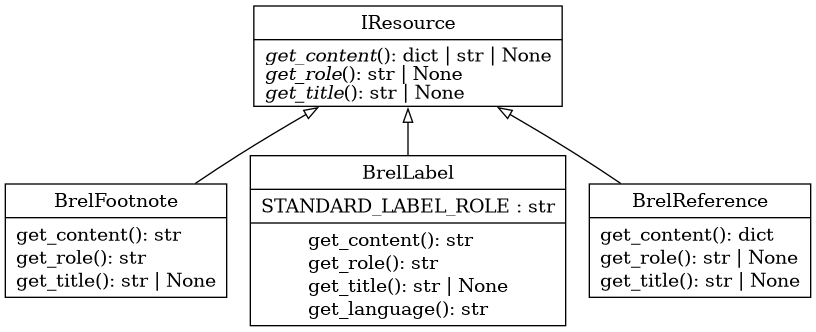
\includegraphics[width=\textwidth]{images/brel_resource_classes.png}
    \caption{UML diagram of the resource classes in Brel}
    \label{fig:brel_resource_classes}
\end{figure}

\subsection{IResource}

% Resources consist of three parts - a role, a title and content.
Resources are comprised of three elements: a role, a title, and content.

% The role acts as a type identifier for the resource.
% For example, even though each XBRL label is represented using a \texttt{BrelLabel} object, 
% there are different types of labels.
% Different types of labels are distinguished using their role.
% As the name suggests, the \texttt{get\_role} method returns the role of the resource. 
The role functions as an identifier for the type of resource.
For instance, while every XBRL label is represented by a \texttt{BrelLabel} object,
labels are differentiated by their role.
The role essentially categorizes the label types,
and the \texttt{get\_role} method retrieves the resource's role.

% Next up is the content of the resource, which is accessed using the \texttt{get\_content} method.
% Usually, the content is a string.
% For references however, the content is embedded XML.
% Since Brel intends to remove any XML dependencies, it returns the embedded XML as a dictionary instead. 
Following this, the resource's content is accessible via the \texttt{get\_content} method.
Typically, the content is textual.
However, for references, the content encompasses embedded XML.
% In alignment with Brel's goal to eliminate XML dependencies,
% this embedded XML is presented as a dictionary instead of its original format.

% The title is a human-readable description of the resource.
% The title, accessed using the \texttt{get\_title} method, is a human-readable description of the resource.
% For labels, the title is often omitted, since the label itself is already short and descriptive.
% However, the content of a resource can be arbitrarily long, which is why XBRL supports titles.
Besides the content, the resource includes a human-readable description, or title.
The \texttt{get\_title} method retrieves the resource's title.

\subsection{Labels and Footnote}

% Footnotes and labels are two types of resources that are used to link to other elements of an XBRL report.
% Even though they have their own classes, they are very similar from an API perspective.
Footnotes and labels represent two distinct resource types utilized to establish connections with other components within an XBRL report.
Despite each having its dedicated class, they are functionally similar from an API perspective.

% Both of them implement the \texttt{IResource} interface.
% The methods \texttt{get\_role}, \texttt{get\_title} and \texttt{get\_content} function virtually the same.
% Unlike their common interface, labels and footnotes have an additional method called \texttt{get\_language}.
% The \texttt{get\_language} method returns the language of the resource.
Both implement the \texttt{IResource} interface,
with the \texttt{get\_role}, \texttt{get\_title}, and \texttt{get\_content} methods operating in a similar manner across both.
Diverging from their shared interface, labels and footnotes introduce an additional method: \texttt{get\_language},
which returns the resource's language.
% The \texttt{get_language} method specifies the resource's language.

\subsection{References}

% References are the third type of resource in XBRL.
% They are used to link XBRL reports to external resources.
% References are represented by the \texttt{Reference} class in Brel and implement the \texttt{IResource} interface.
% They do not have a \texttt{get\_language} method like labels and footnotes do.
% Another difference is that the content of a reference is a dictionary instead of a string.

% Now that we have covered resources, we can finally introduce networks.
References constitute the third resource category within XBRL
and links XBRL reports to external resources.
Like labels and footnotes, references implement the \texttt{IResource} interface.
However, they lack a \texttt{get\_language} method, unlike labels and footnotes.
Moreover, the content of a reference is a dictionary rather than a string.
% facilitating the linkage of XBRL reports to external resources
